% \begin{savequote}[8cm]
% Alles Gescheite ist schon gedacht worden.\\
% Man muss nur versuchen, es noch einmal zu denken.

% All intelligent thoughts have already been thought;\\
% what is necessary is only to try to think them again.
%   \qauthor{--- Johann Wolfgang von Goethe \cite{von_goethe_wilhelm_1829}}
% \end{savequote}

\chapter{Theoretical background}
\label{ch:2-litreview}

\minitoc

This chapter lays out the theoretical framework of the thesis. Section~\ref{sec:the_c_and_p_symmetries_and_their_violation} introduces charge and parity symmetry violation in general, while Section~\ref{sec:cp_violation_in_the_standard_model} covers the description in the Standard Model and the general theory behind charge-parity symmetry violation measurements in charged \B decays. Section~\ref{sec:gamma_with_multibody_d_final_states} focuses on the theory of measurements using $\Bpm\to\D h^\pm$ decays with multi-body \D final states, after which the specific analysis strategy for the measurement described in the thesis is laid out in Section~\ref{sec:strategy_for_lhcb_measurement}.


\section{The C, P and T symmetries and their violation} % (fold)
\label{sec:the_c_and_p_symmetries_and_their_violation}

The concept of symmetry play a fundamental role in modern physics. By Noether's theorem~\cite{}, the simple assumption of invariance of our physical laws under universal temporal and spatial translations leads to the very non-trivial prediction of conserved energy and momentum; 
%
within the field of particle physics, the interactions and dynamics of the Standard Model (SM) follow completely simply from requiring the fundamental particle fields to satisfy a local $U(1)\times SU(2)\times SU(3)$ gauge symmetry~\cite{}; 
%
 and one of the short-comings of the SM,is that it fails to explain the apparent lack of symmetry in our matter-dominated universe.\todo{I'll adjust this paragraph when I've written the introduction.} 
%
Indeed, it is important to experimentally establish the symmetries of our world at a fundamental level, and the degree to which they are broken.

Three discrete symmetries of importance are the symmetries under 
\begin{enumerate}
    \item The charge operator $C$, which conjugates all internal quantum numbers of a quantum state and thus converts particles into their anti-particle counter parts. For example, $C$ transforms the electric charge of a particle state $Q\to-Q$.
    \item The parity operator $P$, which inverts the spatial dimensions of space time: $\vec x \to -\vec x$. As such, it transforms left-handed particle fields into right-handed particle fields and vice versa.
    \item The time-inversion operator $T$, which inverts the temporal dimension of space time: $t\to -t$.
\end{enumerate}
These are fundamentally related by the \emph{CPT} theorem~\cite{} , which states that any Lorentz-invariant Quantum Field Theory (QFT) must be symmetric under the simultaneous application of \emph{all} three operators. However, any one of the symmetries can be broken individually, and experiments have shown the physical laws of our world to violate each of the $C$, $P$, and $T$ symmetries. 

This was first established in 1956, when Chien-Shiung Wu observed parity violation in weak decays of Co-60 nuclei~\cite{}, by carrying out an experiment that was proposed by Yang Chen-Ning and Tsung-Dao Lee~\cite{}. While this experiment established the breaking of $P$ symmetry, it left open the possibility that the physical world would be left invariant under a combination of a charge- and parity inversion; that it was \CP symmetric. However, this was disproved in 1964 when Kronin and Fitch observed that long-lived kaons, which predominantly decay to the \CP-odd $3\pi$ state, could also decay to the \CP-even $\pi\pi$ states~\cite{}. 

Since then \CP violation has been found in the \Bz and \Bpm system by the \babar and \belle collaborations during the early 2000's~\cite{}, and in the \Bs system by \lhcb in 2013~\cite{}; within the last year and a half the first observation of \CP-violation in \Dz decays has been made by the \lhcb collaboration~\cite{}, and most recently evidence for \CP-violation in the neutrino sector has been reported by the T2K collaboration~\cite{}. The observed effects can be divided into distinct classes. The conceptually simplest case is
\begin{enumerate}
    \item \emph{\CP-violation in decay}, where $|A / \bar A| \neq 1$ for a decay amplitude $A$, and the amplitude $\bar A$ of the \CP-conjugate decay. The result is different decay rates in two \CP-conjugate decays
    \begin{align}
        \Gamma (M\to f) \neq \Gamma (\bar M \to \bar f).
    \end{align}
    This type of \CP violation was not established until 1988~\cite{}, 24 years after the first observation of \CP violation, and also this discovery was in $K\to\pi\pi$ decays. 
\end{enumerate}
\CP-violation in decay is the only type possible for charged initial states, and it is thus the main focus of the thesis. Two additional \CP-violating effect are possible for neutral initial states (a situation that will be the main focus of Chapter~\ref{ch:4-KS-CPV}). These effects are
\begin{enumerate}
    \item[2.] \emph{\CP-violation in mixing}, which denotes the case where the mixing rates between the $M^0$ and $\bar M^0$ states differ
    \begin{align}
        \Gamma (M^0 \to \bar M^0) \neq \Gamma (\bar  M^0 \to M^0).
    \end{align}
    The \CP violation first observed by Kronin and Fitch in the neutral kaon sector~\cite{} is (dominantly) of this type. 
    % Experimentally, these effects can also be investigated using final states $f$ $(\bar f)$ specific to $M^0$ $(\bar M^0)$, where \CP violation in mixing will lead to a non-zero value of the asymmetry of "wrong-sign" decays
    % \begin{align}
    %     \frac{\Gamma(M^0 \to \bar f) - \Gamma(\bar M^0 \to f)}{\Gamma(M^0 \to \bar f) + \Gamma(\bar M^0 \to f)}.
    % \end{align}
    
    \item[3.] \emph{\CP-violation in interference between mixing and decay}, which can be present for a neutral initial states $M^0$ decaying into a final state $f$ common to both $M^0$ and $\bar M^0$. The decay rate includes an interference term between two amplitudes: the amplitude for a direct $M^0\to f$ decay and the amplitude for a decay after mixing: $M^0\to\bar M^0\to f$. Even in the absence of the two aforementioned effects, the rates $\Gamma(M^0\to f)$ and $\Gamma(\bar M^0\to \bar f)$ can differ due to the interference term. Such \CP asymmetries have been measured in eg. $\Bz\to J/\psi K$~\cite{} and $\Bs\to J/\psi \phi$ decays~\cite{}.
\end{enumerate}
\CP violation measurements thus have a long, rich, and still-developing history.  

% section the_c_and_p_symmetries_and_their_violation (end)

\section{CP violation in the Standard Model} % (fold)
\label{sec:cp_violation_in_the_standard_model}

All existing measurements of \CP violation in the quark sector are naturally explained in the SM; indeed, the need to explain the observation \CP violation in neutral kaons was a driving force in the development of the model in the first place, when it lead Kobayashi and Maskawa to predict the existence of then-unknown particles in 1973~\cite{} (now known to be the third generation quarks). This section briefly explains the  mechanism behind \CP violation in the SM and then details the current state-of affairs in precision measurements of the fundamental parameter governing the effect: the \CP-violating phase $\gamma$.

\subsection{The CKM matrix and the Unitarity Triangle} % (fold)
\label{sub:the_ckm_matrix}

The SM contains three generations of quarks, each consisting of an up-type quark ($u$, $c$, and $t$) and a down-type quark ($d$, $s$, and $b$). The charged weak interaction of the $W^\pm$ boson couples up and down-type quarks. The quark states that couple to the $W$ are not (a priori) identical to the mass eigenstates, and can be denoted ($u'$, $c'$, and $t'$) and ($d'$, $s'$, and $b'$). A basis for the quark states can be chosen such that the weakly coupling up-quark states are identical to the propagating quark states, $u=u'$, but then the down-type quark stare are different: $d'\neq d$. The two bases of the down-type quarks are related via the CKM matrix\footnote{
    A basis for the quarks can of course be chosen, such that neither the up-quarks or the down-quarks are expressed in their mass eigenstates. In that case the CKM matrix is recovered as $V=U^*_u U_d$, where $U_{u/d}$ is the unitary transformation matrices that brings the $u/d$ quarks into their mass eigenstates.
}
\begin{align}
    \begin{pmatrix}
        d' \\ s' \\ t'
    \end{pmatrix}
    = V \begin{pmatrix}
            d \\ s \\ t
    \end{pmatrix} 
    =
    \begin{pmatrix}
        V_{ud} & V_{us} & V_{ub} \\
        V_{cd} & V_{cs} & V_{cb} \\
        V_{td} & V_{ts} & V_{tb} 
    \end{pmatrix}
    \begin{pmatrix}
            d \\ s \\ t
    \end{pmatrix}.
\end{align}
Thus the Lagrangian terms representing the coupling of a $W^\pm$ boson with a $u$- and a $d$-type quark is
\begin{align}
   \mathcal L_{W^+}= &-\frac{g}{\sqrt{2}}V_{ud} \left(\bar u \gamma^\mu W_\mu^+ d \right)&& \mathcal L_{W^-}=-\frac{g}{\sqrt{2}} V_{ud}^* \left( \bar d \gamma^\mu W_\mu^- u\right)
\end{align}
where $g$ is the weak coupling constant, $\gamma_u$ are the Dirac matrices, and $u$ and $d$ represent the left-handed components of the physical quark states.

The CKM matrix is a unitary complex $3\times3$ matrix, and hence has $3^2=9$ independent, real parameters. However, 5 of these can be absorbed into unphysical phases of the quark states (both mass and weak eigenstates) and hence the matrix has 4 real, physical parameters: 3 mixing angles and a single phase~\cite{Thomson:2013zua}. Chau and Keung~\cite{} proposed the parameterisation
\begin{align}
\begin{split}\label{eq:CK_CKM_matrix}
        V &= 
        \begin{pmatrix}
            1 & 0 & 0 \\ 0 & c_{23} & s_{23} \\ 0 & -s_{23} & c_{23}
        \end{pmatrix}
        \begin{pmatrix}
            c_{13} & 0 & s_{13}e^{-i\delta_{\CP}} \\ 0 & 1 & 0 \\ -s_{13}e^{-i\delta_{\CP}} & 0 & c_{13}
        \end{pmatrix}
        \begin{pmatrix}
            c_{12} & s_{12}  & 0 \\ -s_{12} & c_{12} & 1 \\ 0 & 0 & 1
        \end{pmatrix}
        \\
        &=
        \begin{pmatrix}
            c_{12}c_{13} & s_{12}c_{13} & s_{13}e^{-i\delta_{\CP}} \\
            -s_{12}c_{23}-c_{12}s_{23}s_{13}e^{i\delta_{\CP}} &
            c_{12}c_{23}-s_{12}s_{23}s_{13}e^{i\delta_{\CP}} &
            s_{23}c_{13} \\
            s_{12}s_{23}-c_{12}c_{23}s_{13}e^{i\delta_{\CP}} &
            -c_{12}s_{23}-s_{12}c_{23}s_{13}e^{i\delta_{\CP}} &
            c_{23}c_{13} \\
        \end{pmatrix}
\end{split}
\end{align}
which is the preferred standard by the PDG~\cite{}. Here, $s_{ij}\equiv\sin \theta_{ij}$ and $c_{ij}\equiv\cos \theta_{ij}$ denote the sine and cosine of three rotation angles in quark space; $\theta_{ij}=\theta_C=X$~\cite{} being the usual Cabibbo angle~\cite{}.

The presence of the complex phase $\delta_{\CP}$ in the Lagrangian term of the $W$ coupling causes \CP violation because, as evident from Eq.~\ref{}, if $\delta_{\CP}$ enters the amplitude for some decay mediated by a $W$ boson, $A=|A|e^{i(\delta_0 + \delta_{\CP})}$, then it will enter the \CP conjugate decay amplitude with the opposite sign: $\bar A=|A|e^{i(\delta_0 - \delta_{\CP})}$. In these expressions, $\delta_0$ denotes a \CP conserving phase that is not caused by complex terms in the Lagrangian, but arises due to potential intermediate states in the decay amplitude.\footnote{It is generally true that all phases of a single term in a given amplitude will be convention dependent, but that the phase differences between terms are not.} Usually the underlying mechanism is due to QCD effects, and these \CP conserving phases are therefore generally dubbed \emph{strong} phases, as opposed to the \CP violating \emph{weak} phase of the $W$ coupling~\cite{PDG-CPV-reviw-page-9}. This terminology will be applied throughout the thesis. 

Experimentally, it has been observed that the CKM matrix elements of Eq.~\eqref{eq:CK_CKM_matrix} satisfy $s_{13}\ll s_{23} \ll s_{12}$. This motivates an often used, alternative parameterisation of the matrix, where the elements are expressed as power series in a parameter  $\lambda$ that naturally incorporates this hierarchy: the Wolfenstein parameterisation~\cite{}. The definitions
\begin{align}
    \begin{split}
         s_{12} &\equiv \lambda \\
         s_{23} &\equiv \lambda^2A \\
         s_{13} &\equiv \lambda^3(\rho - i \eta) \\
    \end{split}
\end{align}
are made, after which the unitarity conditions (or Eq.~\ref{eq:CK_CKM_matrix}) determine the remaining elements to any order in $\lambda$.\footnote{Other variants of the Wolfenstein parameterisation do exist~\cite{ahn_wolfenstein_2011}. They all agree at the lowest orders of $\lambda$.} 
To $\mathcal O (\lambda^5)$ the Wolfenstein parameterisation of the CKM matrix is~\cite{wolfenstein_parametrization_1983,https://arxiv.org/pdf/hep-ph/0406184.pdf}
% 
\begin{align}
    V = \begin{pmatrix}
        1-\frac{\lambda^2}{2} -\frac{\lambda^4}{8}&
        \lambda &
        A\lambda^3(\rho - i \eta) \\
        -\lambda+\frac{\lambda^5}{2}A^2(1-2(\rho+i\eta)) &
        1 - \frac{\lambda^2}{2} - \frac{\lambda^4}{8}(1+4A^2) &
        A\lambda^2 \\
        A \lambda^3(1-(\rho + i\eta)(1 - \frac{\lambda^2}{2})) &
        -A\lambda^2 (1- \frac{\lambda^2}{2}(1-2(\rho+i\eta)))&
        1 - \frac{1}{2}A^2\lambda^4
    \end{pmatrix}.
\end{align}{}

The unitarity condition $V^\dagger V = \mathbbm 1$ of the CKM matrix defines 9 relations between the CKM elements of the form
\begin{subequations}
    \begin{align}
    \sum_j V^*_{jq}V_{jq} = 1\quad&,\quad q\in\{d, s, b\} & &\text{along the diagonal} \\
    \sum_j V^*_{jq}V_{jq'} = 0\quad&,\quad q, q'\in\{d, s, b\}, q\neq q' & &\text{off-diagonal}.
\end{align}
\end{subequations}
The off-diagonal conditions constrain three complex numbers to sum to zero, and can thus be visualised as triangles in the complex plane, the so-called unitarity triangles. Of these, the triangle corresponding to the $(d, b)$ elements plays a special role, because all three sides are of the same order of magnitude, $\mathcal O(\lambda^3)$. When expressed in the form
\begin{align}
    \frac{V^*_{ud}V_{ub}}{V^*_{cd}V_{cb}} +  \frac{V^*_{td}V_{tb}}{V^*_{cd}V_{cb}} +1 = 0,
\end{align}
it is often referred to as the singular Unitarity Triangle, illustrated in Fig.~\ref{fig:UT_definition} where the usual names for the three angles are also given.

\begin{figure}[tb]
    \centering
    % \includegraphics[]{}
    \caption{Caption here}
    \label{fig:UT_definition}
\end{figure}

Over-constraining the unitarity triangle by making separate measurements of all sides and angles, in as many different decay channels as possible, is an important, and non-trivial test of the SM. The current experimental constraints are in agreement with the SM predictions, as visualised in Fig.~\ref{fig:UT_constraints}. \todo{Not sure if I should spend time explaining the non-gamma measurements entering?}
The CKM angle
\begin{align}\label{eq:gamma_definition}
    \gamma \equiv \mathrm{arg} (-V_{ud}^{\phantom{*}}V_{ub}^*/V_{cd}^{\phantom{*}}V_{cb}^*)
    = \mathrm{arg} (-V_{cb}^{\phantom{*}}V_{cd}^*/V_{ub}^{\phantom{*}}V_{ud}^*)
\end{align}
is unique among the CKM parameters, in that it can be measured in tree-level processes without significant theoretical uncertainty from lattice QCD calculations~\cite{}.  Because tree-level processes are less likely to be affected by Beyond-Standard-Model (BSM) effects, direct measurements of $\gamma$ can be considered a SM benchmark, which can be compared to estimates based on measurements of other CKM elements that are measured in loop-level processes, and thus are more likely to be affected by BSM effects~\cite{Blanke:2018cya}. 
%This is illustrated with the two plots in Fig.~\ref{fig:ckm_matrix}. 
The current, worldwide combination of direct measurements, published by the CKMFitter group\todo{make sure these are up to data (probably not the case)}, is $\gamma = (72.1^{+5.4}_{-5.7})^\circ $, to be compared with the estimate from loop-level observables of $\gamma = (65.6^{+1.0}_{-3.4})^\circ $~\cite{CKMfitter2015}. Other world averages exist~\cite{HFLAV16,UTfit-UT}, but the overall picture is the same: the ability to constrain BSM physics is currently limited by the uncertainty of the direct measurements. Hence further precision measurements of $\gamma$ are highly motivated. Presently, the precision is driven by time-integrated measurements if direct \CP-violation in $\Bpm\to\D\Kpm$ decays; such a measurement is the topic of this thesis and the topic is treated in detail in the following section. It is also possible to measure $\gamma$ in time-dependent mixing analyses of X, Y, and related decays, by measuring \CP violation in interference between mixing and decay. These modes are expected to provide competitive measurements in the future~\cite{}.

% subsection the_ckm_matrix (end)

\begin{figure}[tb]
    \centering
    % \includegraphics[]{}
    \caption{Caption here}
    \label{fig:UT_constraints}
\end{figure}


\subsection{\texorpdfstring{Measuring $\gamma$ in tree level decays}{Measuring gamma in tree level decays}} % (fold)
\label{sub:_measuring_gamma_in_tree_level_decays}

\begin{figure}[t]
    \centering
        \begin{subfigure}[t]{0.39\textwidth}
        \hspace{0.7cm}
        \begin{tikzpicture}[node distance=1cm and 1cm]
        \coordinate[label=left:$b$] (e1);
        \coordinate[right=of e1] (aux1);
        \coordinate[right=of aux1] (aux2);
        \coordinate[above=of aux2] (aux3);
        \coordinate[right=of aux2,label=right:$c$] (e2);
        \coordinate[right=of aux3] (e3);
        \coordinate[below=of e1] (e4);
        \coordinate[below=of e2] (e5);
        
        %
        \draw[particle] (e1) -- (aux1);
        \draw[longparticle] (3,-0.7) node[right]{$\bar u$} -- (0,-0.7) node[left]{$\bar u$} ;
        \draw[particle] (aux1) node[below]{$V_{cb}$} -- (e2);
        \draw[boson] (aux1) -- (2,1.05);
        \draw[particle] (3,0.7) node[right]{$\bar u$} -- (2,1.05) node[above]{$V_{us}^*$};
        \draw[particle] (2,1.05) -- (3,1.4) node[right]{$s$};

        
\end{tikzpicture}
        \caption{}
        \end{subfigure}
        \begin{subfigure}[t]{0.39\textwidth}
        \hspace{0.7cm}
        \begin{tikzpicture}[node distance=1cm and 1cm]
        \coordinate[] (e1);
        \coordinate[right=of e1] (aux1);
        \coordinate[right=of aux1] (aux2);
        \coordinate[below=of aux2] (aux3);
        \coordinate[right=of aux2] (e2);
        \coordinate[right=of aux3] (e3);
        \coordinate[below=of e1] (e4);
        \coordinate[below=of e2] (e5);
        
        %
        \draw[particle] (e1) node[left]{$b$} -- (aux1);
        \draw[longparticle] (3,-2.1) node[right]{$\bar u$} -- (0,-2.1) node[left]{$\bar u$};
        \draw[particle] (aux1) node[above]{$V_{ub}$}-- (e2) node[right]{$u$};
        \draw[boson] (aux1) -- (2,-1.05);
        \draw[particle] (2,-1.05) node[below]{$V_{cs}^*$} -- (3,-1.4) node[right]{$s$};
        \draw[particle] (3,-0.7) node[right]{$\bar c$} -- (2,-1.05);

        
\end{tikzpicture}
        \caption{}
        \end{subfigure}
        \caption{Tree level Feynman diagrams describing (a) ${\Bm\rightarrow \Dz \Km}$ and (b) ${\Bm\rightarrow \Dzb \Km}$ decays. The electro-weak phase difference between the two decays is $\Delta\phi = 
\text{arg}\left( {V_{cb}V_{us}^*}/{V_{ub}V_{cs}^*} \right)\simeq\gamma$.}
        \label{fig:feynman_diagrams}
    
\end{figure}

The phase $\gamma$ can be measured in tree-level processes with interference between $b\to c s \bar u$ and $b\to \bar c s u$ transitions. The canonical example, also the subject of this thesis, is based on measurements sensitive to interference between the $\Bpm\to\Dz\Kpm$ and $\Bpm\to\Dzb\Kpm$ decay amplitudes. As illustrated in Fig.~\ref{fig:feynman_diagrams} for the case of \Bm decays, the electro-weak phase difference between the two decays is $\Delta\phi = 
\text{arg}\left( {V_{cb}^{\phantom{*}}V_{us}^*}/{V_{ub}^{\phantom{*}}V_{cs}^*} \right)$. While $\Delta\phi$ is not identical to the definition of $\gamma$ in Eq.~\eqref{eq:gamma_definition}, the ratio of the involved CKM matrix elements is~\cite{grossman_effects_2014}
\begin{align}
-\frac{V_{cd}^*/V_{ud}^*}{V_{us}^*/V_{cs}^*} 
&= - \frac{
-\lambda [1-\frac{\lambda^4}{2}A^2(1-2(\rho-i\eta))](1-\frac{\lambda^2}{2}-\frac{\lambda^4}{8}(1+4A^2))
}
{\lambda(1-\frac{\lambda^2}{2}-\frac{\lambda^4}{4})} \notag \\
&= 1 - \lambda^4 A^2  (1 - 2(\rho -i\eta)) + \mathcal O(\lambda^5). 
\end{align}
The ratio equals unity to $\mathcal O(\lambda^4)\simeq 2.6\times 10^{-3}$, and thus $\Delta\phi\simeq\gamma$ is a good approximation within current experimental uncertainties. For the remainder of this thesis the approximation will be used without further comment. The diagrams in Fig.~\ref{fig:feynman_diagrams} describe the leading order contributions to the two amplitudes
\begin{subequations}\label{eq:B_amplitudes}
\begin{align}
\begin{split}    
    A[\Bm\to\Dz\Km] &\equiv A_B \\
    A[\Bm\to\Dzb\Km] &\equiv \bar A_B  \equiv r_B A_B e^{i(\delta_B - \gamma)},
\end{split}
\end{align}
where the last equality introduces two new parameters: the amplitude magnitude ratio $r_B\equiv |\bar A_B |/|A_B|$, and $\delta_B$, the strong-phase difference between the decay amplitudes.  Since all \CP-violation is attributed to the electro-weak phase in the SM, the \CP-conjugate decay amplitudes are~\cite{gronau_determining_1991}
\begin{align}
\begin{split}    
    A[\Bp\to\Dzb\Kp] &= A_B \\
    A[\Bp\to\Dz\Kp]  &= \bar A_B = r_B A_B e^{i(\delta_B + \gamma)}.
\end{split}
\end{align}
\end{subequations}
In an experimental setting, the \Dz and \Dzb mesons are reconstructed in some final state, $f$ or its \CP-conjugate $\bar f$. In analogy with the \Bpm decays, the \D decay amplitude can be related\footnote{In this notation $\delta_D$ is thus phase of the suppressed \D-decay amplitude minus the phase of the favoured \D-decay amplitude. This is the opposite convention to that used in the \lhcb measurements with the ADS technique~\cite{}, but aligns with the notation used in the literature on $\gamma$ measurements in $\D\to\KS\pip\pim$ decays~\cite{}.} 
\begin{align}
\begin{split}\label{eq:D_amplitudes}
    A[\Dz\to f] &= A[\Dzb\to \bar f] = A_D \\ 
    A[\Dzb \to f] &= A[\Dz \to \bar f] = r_D A_D e^{i\delta_D}.
\end{split}
\end{align}
where the assumption has been made that there is no \CP violation in the \D decays, and $\delta_D$ denotes a \CP-conserving strong-phase difference. While \CP-violation in \D decays has recently been measured~\cite{}, the size of the effect is small and it is considered negligible in this thesis. Based on Eqs.~\ref{eq:B_amplitudes}~and~\eqref{eq:D_amplitudes}, the decay rates of \Bp and \Bm mesons into the possible final states can be seen to satisfy 
\begin{subequations}\label{eq:rate_equations}
\begin{align}
    \Gamma(\Bm \to \D(\to f)\Km) & \propto 
    1 + r_D^2 r_B^2 + 2 r_B r_D \cos\left[\delta_B + \delta_D - \gamma\right], \label{eq:rate_Bm_f}\\
    \Gamma(\Bp \to \D(\to \bar f)\Kp) & \propto 
    1 + r_D^2 r_B^2 + 2 r_B r_D \cos\left[\delta_B + \delta_D + \gamma\right], \label{eq:rate_Bp_fbar}\\
    \Gamma(\Bm \to \D(\to \bar f)\Km) & \propto
    r_D^2 + \phantom{1}r_B^2 + 2 r_B r_D \cos\left[\delta_B - \delta_D - \gamma\right], \label{eq:rate_Bm_fbar}\\
    \Gamma(\Bp \to \D(\to f)\Kp) & \propto
    r_D^2 + \phantom{1}r_B^2 + 2 r_B r_D \cos\left[\delta_B - \delta_D + \gamma\right]. \label{eq:rate_Bp_f} 
\end{align}
\end{subequations}
The processes in Eqs.~\eqref{eq:rate_Bm_f}~and~\eqref{eq:rate_Bp_fbar} are \CP-conjugate and it is clear how, in the typical case where $\delta_B+\delta_D\neq 0$,  a non-zero value of $\gamma$ leads to \CP violation in the form of differing decay rates. The same is true for the processes in Eqs.~\eqref{eq:rate_Bm_fbar}~and~\eqref{eq:rate_Bp_f}. Depending on the choice of \D final state, these expressions can be used to relate $\gamma$ to various observables that are experimentally accessible. This thesis concerns the choice $f=\KS\pip\pim$ or $f=\KS\Kp\Km$, where the terms related to the \D decay all have a non-trivial variation over the phase space of the decay. However, it is useful to first analyse the simpler case where $f$ is a two-body state. 

The simplest case is when $f$ is chosen to be a \CP eigenstate, so that $f=\pm\bar f$ and the rate equations~of~\eqref{eq:rate_Bm_f}--\eqref{eq:rate_Bp_f} simplify, because $r_D=1$ and $\delta_D\in\{0,\pi\}$. Measurements of $\gamma$ in such decay modes are denoted GLW measurements, after  Gronau, London, and Wyler who described the approach in the early 90ies~\cite{gronau_determining_1991,gronau_how_1991}. Experimentally it is preferable to measure yield ratios rather than absolute rates, and the observables of interest are thus the \CP asymmetry
\begin{subequations}\label{eq:GLW_observables}
\begin{align}
\begin{split}
    A_{\CP=\pm1} &= \frac{\Gamma[\Bm\to D_{\CP}\Km] - \Gamma[\Bp\to D_{\CP}\Kp]}{\Gamma[\Bm\to D_{\CP}\Km] + \Gamma[\Bp\to D_{\CP}\Kp]} \\
    &= \frac{\pm r_B \sin \delta_B \sin \gamma}{1 + r_B^2 \pm 2 r_B \cos \delta_B \cos \gamma},
\end{split}
\end{align}
as well as the ratio
\begin{align}
\begin{split}
    R_{\CP=\pm 1} &= 2\frac{\Gamma[\Bm\to D_{\CP}\Km] + \Gamma[\Bp\to D_{\CP}\Kp]}{\Gamma[\Bm\to \Dz\Km] + \Gamma[\Bp\to \Dzb\Kp]} \\
    &=  1 + r_B^2 \pm 2 r_B \cos \delta_B \cos \gamma.
\end{split}
\end{align}
\end{subequations}
In practice, $A_{\CP}$ and $R_{\CP}$ are obtained from measured yield ratios that are corrected with appropriate branching fractions. A measurement of $A_{\CP}$ and $R_{\CP}$ alone is not sufficient to determine the underlying physics parameters $(\gamma, r_B, \delta_B)$, and this is not solely due to the number of parameters exceeding the number of constraints: the equations also allow for multiple, ambiguous solutions for $(\gamma, \delta_B)$. 
%When combined with additional measurements that constrain $r_B$, measurements of $A_{\CP}$ and $R_{\CP}$ put quite stringent constraints on $\delta_B$ and $\gamma$, albeit with multiple, ambiguous solutions. For a given $\delta_B$ two different solutions exist for $\gamma$, and furthermore the equations are invariant under the exchange $\delta_B \leftrightarrow \gamma$, as well as the simultaneous transformation $(\gamma, \delta_B) \to (\gamma + \pi, \delta_B + \pi)$. Typical constraints on $(\gamma, r_B, \delta_B)$ for a measured set of GLW observables are illustrated in Fig.~\ref{fig:typical_GLW_constraints}, for observables corresponding to $(\gamma, r_B, \delta_B) = (75^\circ, 0.1, 130^\circ)$, which is fairly representative of the current, experimental average.\footnote{A full interpretation of $A_{\CP}$ and $R_{\CP}$ in terms of the underlying physics parameters also needs to take secondary effects, such as \D-mixing, into account. Such effects are ignored in this exposition, where the point is simply to illustrate the fundamental principles of the measurement strategy.} 
One way to break the ambiguity, first noted in the original paper~\cite{gronau_determining_1991}, is to make further measurements in additional \B decays. These can be described with the  formalism described above, but will not share the same ambiguous solutions because $(r_B, \delta_B)$ are unique to a given \B decay. Another method is to analyse \D decay final states that are not \CP eigenstates.


\begin{figure}[tb]
    \centering
    % \includegraphics[]{}
    \caption{Caption here}
    \label{fig:typical_GLW_constraints}
\end{figure}


In the XX analysed an alternative choice of \D final states: a simultaneous analysis of a Cabibbo-favoured (CF) decay $\Dz\to f$ and the doubly-Cabibbo-suppressed (DCS) decay $\Dz\to \bar f$ into the \CP conjugate final state. The classical example is to take $f=\Km\pip$ and $\bar f = \pim\Kp$. The relative suppression means that the $r_D$ of Eq.~\eqref{eq:rate_equations} is small, typically of the same order of magnitude as $r_B$, and thus the \CP asymmetry of the suppressed decay is $\mathcal O(1)$:
\begin{subequations}\label{eq:ADS_observables}
\begin{align}
\begin{split}
    A_{ADS(\bar f)} &= \frac{\Gamma[\Bm\to D(\to\bar f)\Km] - \Gamma[\Bp\to D(\to f)\Kp]}{\Gamma[\Bm\to D(\to\bar f)\Km] + \Gamma[\Bp\to D(\to f)\Kp]} \\
    &= \frac{r_Dr_B \sin (\delta_B - \delta_D) \sin \gamma}{r_D^2 + r_B^2 + 2 r_Dr_B \cos (\delta_B - \delta_D) \cos \gamma}.
\end{split}
\end{align}
The large \CP asymmetry is a prime feature of the ADS method. However, also the suppressed-to-favoured yield ratio is sensitive to the physics parameters of interest:
\begin{align}
\begin{split}
    R_{ADS(\bar f)} &= \frac{\Gamma[\Bm\to D(\to\bar f)\Km] + \Gamma[\Bp\to D(\to f)\Kp]}{\Gamma[\Bm\to D(\to f)\Km] + \Gamma[\Bp\to D(\to \bar f)\Kp]} \\
    &= \frac{r_B^2 + r_D^2 + 2 r_Dr_B \cos (\delta_B - \delta_D) \cos \gamma}{1 + r_D^2 r_B^2 + 2 r_Dr_B \cos (\delta_B + \delta_D) \cos \gamma}.
\end{split}
\end{align}
\end{subequations}
The interpretation of $A_{ADS}$ and $R_{ADS}$ in terms of $(\gamma, r_B, \delta_B)$ requires knowledge of the $r_D$ and $\delta_D$ parameters, but these can be measured independently~\cite{}. In general, the constraints from a single set of ADS observables suffer the same ambiguities as in the GLW case. However, unlike the GLW case, each \D decay mode provides an independent set of constraints, because the parameters related to the \D decay vary. 

The discussion of this section has centred on the classical case of $\Bpm\to D\Kpm$ decays with a two-body \D final state. With minor modifications the techniques have been used to make measurements of $\gamma$ in \Bz decays~\cite{}, with \B decay final states including excited \D mesons~\cite{}, excited kaons~\cite{}, or pions~\cite{}. The decay $\Bpm\to D \pipm$ also is also \CP-violating, although the effect is much smaller than in the $\Bpm\to D\Kpm$ decay, because $r_B^{\Dpi}\simeq 0.005 \sim \mathcal O(\lambda^X)$, whereas $r_B^{\DK}\simeq 0.1 \sim \mathcal O(\lambda^X)$. Furthermore, it is possible to use multi-body \D final states~\cite{}. However, in some cases, a better precision can then be obtained by exploiting phase-space dependent decay rates. This is the topic of the next section.


% subsection _measuring_gamma_in_tree_level_decays (end)

\section{\texorpdfstring{Measuring $\gamma$ using multi-body D final states}{Measuring gamma using multi-body D final states}} % (fold)
\label{sec:gamma_with_multibody_d_final_states}


In multi-body \D decays, the $r_D$ and $\delta_D$ parameters of the fundamental rate equations in Eq.~\eqref{eq:rate_equations} vary over the phase space of the \D decay. This section describes a model-independent approach to measure $\gamma$ in $\B\to\D(\to\KS\pip\pim)h^\pm$ decays by exploiting this variation. The theory is identical for $\D\to\Ks\Kp\Km$ decays, and similar ideas have been proposed for the $\D\to\KS\pip\pim\piz$~\cite{} and $\D\to2\pip2\pim$ modes~\cite{}. First, however, the formalism for describing amplitudes of multi-body decays is briefly reviewed.


\subsection{Dalitz plots and the phase space of multibody decays} % (fold)
\label{sub:the_phase_space_of_multibody_decays_and_dalitz_plots}

In general, the phase space of the $n$-body decay $P\to p_1 + p_2 + ... + p_n$ consists of $n$ four momenta, with a total of $4n$ components. The requirement that each of the final state particles is on-shell provides $n$ constraints on these components, and energy-momentum conservation removes a further 4 degrees of freedom. If the original particle $P$ is s \emph{scalar}, the decay is isotropic, which removes an additional 3 degrees of freedom, leaving the total number of degrees of freedom at $3n-7$. For the specific case of three-body decays, the available phase space can thus be parameterised with only two parameters. A practical and often used choice is the invariant masses
\begin{align}
    s_{12} &= m^2(p_1p_2) = (p_1^\mu+p_2^\mu)^2, & s_{13} &= m^2(p_1p_3) = (p_1^\mu+p_3^\mu)^2.
\end{align}
The choice of particle pairs is arbitrary, and the coordinates easily related
\begin{align}
    m^2_P + m^2_{p_1} + m^2_{p_2} + m^2_{p_3} = m^2(p_1p_2) + m^2(p_1p_3) + m^2(p_2p_3).
\end{align}
A scatter plot of $(s_{12}, s_{13})$ values for a sample of particle decays is denoted a Dalitz plot~\cite{}. It has the very useful feature that the presence of (narrow) resonances in the decay leads to visible bands in the scatter plot. Figure~\ref{} shows an example of a Dalitz plot for $\D\to\KS\pip\pim$ decays in which the $K^*(892)^\pm$ and $\rho(770)$ resonances are clearly visible. The plot shows the sample of $\Bm\to\D\pim$ decays used to make the measurement described in Chapter~\ref{ch:5-GGSZ-measurement} and thus the \D meson is in a superposition of \Dz and \Dzb states (as detailed in the following section). 

In terms of the coordinates of Eq.~\eqref{} the differential decay rate is given by~\cite{PDG-kinematics-review}
\begin{align}
    \text d \Gamma = \frac{1}{32(2\pi)^3 m^3_P} |\mathcal M|^2 \,\text d s_{12} \text d s_{13},
\end{align}
where $\mathcal M$ is the QFT matrix element, or total decay amplitude, corresponding to the decay. In general, it is not possible to calculate $\mathcal M$ from first principles. Instead, a model is defined with an empirically well motivated form, in which a number of free parameters must be determined experimentally. The simplest case is that of an \emph{isobar} model, where it is assumed that the full decay can be decomposed into consecutive two-body decays of the form $P \to R_{12} (\to p_1 + p_2) p_3$. Thus, $\mathcal M$ is expressed as a non-resonant constant amplitude term, $k_{NR}$, plus a sum of resonance terms
\begin{align}\label{eq:amplitude}
    \mathcal M (s_{12}, s_{13}) = k_{NR} + \sum_r k_r \mathcal M^r(s_{12}, s_{13}).
\end{align}
The exact form of the $\mathcal M^r$ function depends on the resonance in question. A detailed review can be found in eg. Ref.~\cite{}. The isobar formalism breaks down when resonances in the decay are not well separated. In this case, models of the form in Eq.~\eqref{} can still be employed, if the contribution from overlapping resonances are collected in a single term. An example of such a model, is the amplitude model for $\Dz\to\KS\pip\pim$ decays developed by the Belle collaboration for a measurement of the CKM angle $\beta$ in 2018~\cite{}. In this model, individual terms are included for $\Dz\to\Kstar(\to\KS\pi^\pm)\pimp$ decays, whereas the resonant behaviour of the $\pi\pi$ decay products is modelled with the so-called $K$-matrix formalism~\cite{}. The amplitude and phase of $\mathcal M$ as predicted by this model are shown in Fig.~\ref{}.


% subsection the_phase_space_of_multibody_decays_and_dalitz_plots (end)


\subsection{\texorpdfstring{The GGSZ method to measure $\gamma$}{The GGSZ method to measure gamma}} % (fold)
\label{sub:the_ggsz_method_to_measure_gamma}

% subsection the_ggsz_method_to_measure_gamma (end)
The non-trivial phase-space dependence of the $\D\to\KS\pip\pim$ decay amplitude can be exploited to measure $\gamma$ with $\Bpm\to \D\Kpm$ or $\Bpm\to \D\pipm$ decays. For this specific decay, \sm and \sp are used to described the Dalitz coordinates $m^2(\KS\pim)$ and $m^2(\KS\pip)$, respectively, and the \D decay amplitude is a function of these coordinates
\begin{align}\label{eq:ADDb_definition}
\ADorDbS (\smpLong)= A(\DorDbar^0\to K^0_\text{S} \pi^+\pi^-).
\end{align}
To a good approximation the \KS meson is a \CP eigenstate, meaning that the $\KS\pip\pim$ state is self-conjugate. Assuming this approximation to be exact, and that \CP violation in the \D decay is negligible, the \D decay amplitude satisfies the symmetry relation
\begin{align}\label{eq:KS_symmetry}
     \ADbS(\sm, \sp)=\ADS(\sp, \sm).
 \end{align} 
 The impact of the \KS meson \emph{not} being an exact \CP eigenstate is treated in detail in Chapter~\ref{ch:4-KS-CPV}. In order to simplify equations, the short-hand notation 
 \begin{align}
     (s_{-+})&=(s_-,s_+), &(s_{+-})&=(s_+,s_-)
 \end{align} will be employed for the remainder of this thesis, so that the relation in Eq.~\eqref{eq:KS_symmetry} can be expressed as $\ADbS(\smp)=\ADS(\spm)$. Thus, the rate equations of Eq.~\eqref{eq:rate_equations} for the $\D\to\KS\pip\pim$ decay mode are
 \begin{subequations}
\begin{align} \label{eq:Gamma_Bminus}
    \rm {d} \Gamma^-(\smp) &\propto |\cASm|^2 = |\AB|^2|\AKS|^2 \notag \\
    &\qquad\times\left[|\ADS(\smp)|^2 + \rB^2 |\ADS(\spm)|^2 + 2\rB |\ADS(\smp)||\ADS(\spm)|\right .
    \notag \\
    &\quad\qquad \left. \times \left(\cos[\delta_D(\smp)]\cos[\dB-\g]+\sin[\delta_D(\smp)]\sin[\dB-\g]\right)\right], \\
    \rm {d} \Gamma^+(\smp) &\propto |\cASp|^2 = |\AB|^2|\AKS|^2 \notag \\
    &\qquad\times\left[|\ADS(\spm)|^2 + \rB^2 |\ADS(\smp)|^2 + 2\rB |\ADS(\smp)||\ADS(\spm)|\right .
    \notag \\
    &\quad\qquad \left. \times \left(\cos[\delta_D(\smp)]\cos[\dB+\g]-\sin[\delta_D(\smp)]\sin[\dB+\g]\right)\right].
\end{align}
\end{subequations}
Here, $\delta_\D(\smp) = \phi_D(\smp) - \phi_D(\spm) = - \delta_D(\spm)$, where $\phi_D(\smp)$ denotes the complex phase of the $\ADS(\smp)$ amplitude, and a standard trigonometric relation have been employed to factorise the terms depending on the complex phases of the \B and \D decays. It can be seen that in the case where $\gamma=0$ the \Bp and \Bm decay rates are symmetric if the Dalitz coordinates are exchanged: $\Gamma^+(\sm, \sp)=\Gamma^-(\sp, \sm)$. The presence of \CP violation in the \B decay breaks the symmetry. Therefore it is possible to measure \g (and the nuisance parameters \rB and \dB) from the phase-space distribution of $\Bpm\to\D(\to\KS \pi^+ \pi^-)\Kpm$ decays, given knowledge of $\ADS(\smp)$. A series of measurements of \g have been made that use amplitude models of the \D decay \cite{BABAR2005,BABAR2008,BABAR2010, BELLE2004,BELLE2006,BELLE2010,LHCb-PAPER-2014-017,LHCb-PAPER-2016-007}. However, the topic of this thesis is a model-independent measurement\todo{Here is where the discussion of model-dependent vs model-independent should go.}


\subsection{A model-independent approach} % (fold)
\label{sub:a_model_independent_approach}


The phase-space distribution can be analysed in a model-independent way, if the $\D$-decay phase space is split into regions, or bins, an the $\B$ decay yield in each bin determined experimentally. The binned approach was featured in the original GGSZ paper~\cite{} and the model-independent approach developed further in Refs.~\cite{}. A measurement of $\gamma$ using this approach is the main topic of the thesis. This section describes the fundamental principle, whereas the details pertaining to the exact experimental approach are delegated to Section~\ref{}. 

\begin{figure}[tb]
     \centering
     % \includegraphics[]{}
     \caption{Caption here}
     \label{fig:GGSZ_bin_principle}
 \end{figure} 

The amplitude symmetry of Eq.~\eqref{eq:KS_symmetry} is exploited by defining $2N$ bins to be symmetric symmetric around the $\sm=\sp$ diagonal of the Dalitz plot, numbered $i=-N$ to $N$ (omitting zero) such that if the point $(\sm, \sp)$ is in bin $i$, then $(\sp, \sm)$ is in bin $-i$, and by convention $i>0$ for bins where $s_- >s_+$. The principle is illustrated in Fig.~\ref{fig:GGSZ_bin_principle}, but the binning schemes used in actual measurements are more complicated. The decay rates in Eq.~\eqref{} can be integrated over such bins, and give the bin yields
\begin{align}
\begin{split}    \label{eq:base_GGSZ_yields}
    N^-_i &\propto h^- \left[\Ki + \rB^2\Kmi + 2\sqrt{\Ki\Kmi}\left(\ci\xm+\si\ym\right)\right], \\
    N^+_i &\propto h^+ \left[\Kmi + \rB^2\Ki + 2\sqrt{\Ki\Kmi}\left(\ci\xp-\si\yp\right)\right],
\end{split}
\end{align}
where the parameters describing the \B decay have been expressed in terms of the observables
\begin{align}
    \xpm &= \rB \cos (\dB \pm \g), & \ypm &= \rB \sin (\dB \pm \g),
\end{align}
 and a number of phase-space integrated quantities related to the \D-decay have been introduced. The $K_i$ parameters denote fractional yield of a flavour-tagged \Dz decaying into bin $i$, defined as
\begin{align}\label{eq:base_ki}
    K_i &= \frac{1}{N_K}\int_i\text{d}s^2 |\ADS(\smp)|^2, &
    N_K &=\int\text{d}s^2 |\ADS(\smp)|^2,
\end{align}
where $\int_i \text d s^2$ denotes integration over bin $i$ of the Dalitz plot. The \ci and \si denote the amplitude-weigthed average of $\cos \delta_D(\smp)$ and $\sin \delta_D(\smp)$ over bin $i$
\begin{align}\label{eq:ci_si}
\begin{split}
    \ci &= \frac
    {\int_i \text{d}s^2 |\ADS(\smp)||\ADS(\spm)|\cos[\delta_D(\smp)]}
    {\sqrt{\int_i \text{d}s^2 |\ADS(\smp)|^2}\sqrt{\int_i \text{d}s^2 |\ADS(\spm)|^2}}, \\
    \si &= \frac
    {\int_i \text{d}s^2 |\ADS(\smp)||\ADS(\spm)|\sin[\delta_D(\smp)]}
    {\sqrt{\int_i \text{d}s^2 |\ADS(\smp)|^2}\sqrt{\int_i \text{d}s^2 |\ADS(\spm)|^2}}.
\end{split}
\end{align}
By the symmetry properties of $\delta_D(\smp)$ these parameters satisfy ${c_i=c_{-i}}$ and ${s_i=-s_{-i}}$. The normalisation constants $h^+$ and $h^-$ are identical in the ideal case, but it is convenient to keep define them separately for practical reasons: depending on the experimental setup, there may be overall production and detection asymmetries that affect the total signal yields. An experimental analysis can be made insensitive to these effects because they can be absorbed into the normalisation constants, as long as they are constant over the \D-decay phase space. This comes at the cost that the information on \xpm and \ypm from the overall \CP asymmetry is lost, but Section~\ref{sub:relation_to_glw_and_ads_measurements} will show that the loss in precision is minimal.

Thus, for a set of 2$N$ bins, the bin yields of Eqs.~\eqref{eq:base_GGSZ_yields} provide $4N$ constraints on a total of $4N+6$  parameters: $(h^\pm, K_i, c_i, s_i, x_\pm, y_\pm)$. However, the $K_i$, $c_i$, and $s_i$ parameters relate only to the \D decay, and can thus, in principle, be measured in independent experiments. With such external inputs a measurement of the $\Bpm\to D(\to\KS\pip\pim)\Kpm$ yields in a set of bins can be used to constrain \xpm and \ypm, and thereby $(\gamma, r_B, \delta_B)$. The measurement presented in this thesis determines the $K_i$ parameters directly, but uses externally measured values of \ci and \si as input, as measured in quantum correlated \D decays by the CLEO~\cite{} and BESIII~\cite{} collaborations. Because these measurements are the foundation of the approach, they are described in some detail in the following section.

\subsection{Measuring strong-phase inputs at charm factories} % (fold)
\label{sub:measuring_strong_phase_inputs_at_charm_factories}

The strong-phase parameters $c_i$ and $s_i$ have been measured by the CLEO and BESIII collaborations, using quantum correlated \Dz\Dzb pairs from decays of the $\psi(3770)$ resonance state, itself produced in $e^+e^-$ collisions at the resonance energy. The $\psi(3770)$ has quantum-number $C=-1$, which is conserved in the strong decay into two \D mesons, and thus the two \D mesons are produced in an anti-symmetric wave function. By observing the decay of one \D meson into a specific final state, say a \CP eigenstate, the quantum state of the other \D meson can be determined. The measurement is based on decays where both \D decays are reconstructed, one in the $\KS\pip\pim$ final state, the other in one of several different tag categories. The main principles are outlined below, but most experimental considerations and implementation details are left out for the sake of brevity.

The simplest case is when one \D meson decays into a final state that uniquely tags the flavour, such as $\Dzb\to\Kp e^-\bar\nu_e$. In that case, the \D meson decaying to $\KS\pip\pim$ is known to be in the \Dz state and the decay rate is simply determined by $\ADS: \Gamma(\smp)\propto |\ADS(\smp)|^2$. This allows for a measurement of the $K_i$ parameters.

If one \D meson is reconstructed in a \CP-even state, eg. $\Kp\Km$, or a \CP-odd state, eg. $\KS\piz$, the \D meson decaying to $\KS\pip\pim$ is known to be in a state of opposite \CP. Thus, for a tag-decay of $\CP=\pm1$ the decay rate has the form
\begin{subequations}
\begin{align}\label{eq:CP_cisi}
    \Gamma_{\CP=\pm1} \propto \left| \ADS(\smp) \mp \ADS(\spm)\right|^2
\end{align}
and the bin yields will be given by
\begin{align}
    M_i^\pm \propto K_i + K_{-i} \mp 2 \sqrt{K_i K_{-i}}c_i.
\end{align}
\end{subequations}
Thus a simultaneous analysis of flavour and \CP tagged decays allow for a determination of the $K_i$ and \ci parameter sets.

Finally, the case where both \D mesons, for now denoted \D and $\D'$, decay into the $\KS\pi\pi$ final state can be considered. The total amplitudes have contributions from the case where \D is in the \Dz state and $\D'$ is in the \Dzb state, as well as the opposite flavour assignment. Thus the decay rate satisfies
\begin{subequations}\label{eq:Kspipi_cisi}
\begin{align}
    \Gamma_{\CP=\pm1} \propto \left| \ADS(\smp)\ADS(\spm') + \ADS(\spm)\ADS(\smp')\right|^2
\end{align}
where \smp denotes the Dalitz-plot coordinates of the \D meson, and $\smp'$ those of the $\D'$ meson. Defining $M_{ij}$ to be the yield of decays where the \D decay is in bin $i$ and the $\D'$ in bin $j$, the bin yields satisfy
\begin{align}
    M_{ij} \propto K_iK_{-j} + K_jK_{-i} - 2\sqrt{K_iK_{-i}K_jK_{-j}}\left(c_ic_j + s_is_j\right).
\end{align}
\end{subequations}
Thus, analysing these decays in addition to the \CP and flavour tagged decays provide information on all of $K_i$, \ci, and \si. Note, however, that Eqs.~\eqref{eq:CP_cisi} and \eqref{eq:Kspipi_cisi} are invariant under the transformation $\delta_D\to-\delta_D$\todo{Where exactly is this phase sign know from? Is the overall sign not arbitrary in amplitude models?}. In practice, the analysis is extended in a number of ways to enhance the statistics: using "flavour-tag" states that are not exact flavour tags, such as $\Km\pip$, using self-conjugate multi-body \D-decay final states that are not exact \CP eigenstates, such as $\pip\pim\piz$, and using the \KL\pip\pim final state as well. However, the main principles are the same as described above.

The measurements of \ci and \si are made for a range of different binning schemes. It was noted already in Ref.~\cite{} that a rectangular binning scheme, such as the example in Fig.~\ref{}, does not provide the optimal sensitivity to $\gamma$. A better sensitivity can be obtained if the bins are defined such that $\delta_\D$ is approximately constant over a given bin, by defining bin $i$ out of $N$ via the condition
\begin{align} \label{eq:equal_binning_definition}
    \text{bin}_i = \left\{ (s_-, s_+)\quad  | \quad 2\pi (i-3/2)/N \,<\, \delta_D(\sm, \sp) \,<\, 2\pi \times (i-1/2)/N  \right\}.
\end{align}
In practice, the binning scheme is defined by splitting the \D-decay phase-space into quadratic \emph{micro bins} with a width of X $(\gevcc)^2$ and assigning a bin number to each micro bin via the condition in \eqref{eq:equal_binning_definition} as evaluated in an amplitude model of choice. The obtained binning scheme when using an amplitude model developed by the \babar collaboration in 2008~\cite{} is shown in Fig.~\ref{}. In Ref~\cite{} it was also shown that the binning can be even further optimised for sensitivity. The suggested figure of merit is
\begin{align}
    Q^2 = \frac
    {\sum_i \left(\frac{1}{\sqrt{N_i^{\B}} }\frac{\text d N_i^{\B}}{\text d x} \right)^2 + \left(\frac{1}{\sqrt{N_i^{\B}}} \frac{\text d N_i ^{\B}}{\text d y} \right)^2}
    {\int \text d s^2 \left[\left(\frac{1}{|\Gamma^{\B}(\smp)|}\frac{ \text d |\Gamma^{\B}(\smp)|^2 }{ \text d x}\right)^2 + \left(\frac{1}{|\Gamma^{\B}(\smp)|}\frac{ \text d |\Gamma^{\B}(\smp)|^2 }{ \text d y}\right)^2 \right]}
\end{align}
which quantifies the statistical sensitivity for a given binning, relative to the one achievable in an unbinned analysis. The CLEO collaboration defined an \emph{optimal} binning scheme by an iterative procedure where, starting from the equal binning scheme, a micro-bin is randomly reassigned new bin numbers in each step, and a step accepted if $Q^2$ increases. The optimisation is done for the case where $x=y=0$ and thus $Q^2$ simplifies to $Q^2_{x=y=0}=\sum_i N_i^{x=y=0}(c_i^2+s_i^2)/N_{total}^{x=y=0})$. The resulting binning scheme is shown in Fig.~\ref{}. An additional binning scheme is defined, denoted the \emph{modified optimal} scheme and shown in Fig.~\ref{}, where the $Q^2$ figure of merit is modified to take into account the presence of backgrounds~\cite{}. The modified optimal binning scheme has proven beneficial to use in measurements with small signal yields~\cite{}, but is not employed in the present thesis.


While the \emph{definition} and \emph{optimisation} of these binning schemes depend on knowledge of $\ADS(\sm, \sp)$ via an amplitude model, it is important to note that no model information is used when the binning schemes are used in the subsequent measurements of strong-phases\footnote{With the exception of minimal model-dependence introduced when the $\KL\pip\pim$ final state is employed to constrain the \si parameters by the \D-factories~\cite{}, the impact of which is well under control.} or \CP-observables. Therefore the measurements will not be biased by any modelling imperfections, although the obtained precision might be lower than expected. 

Both the CLEO and BESIII collaborations have measured the values of \ci and \si for the equal, optimal, and modified optimal binning schemes. The results are shown in Figs.~\ref{}~and~\ref{}, where they are also compared to the expectation from the latest amplitude model. The measurements presented in this thesis are based on a combination of the BESIII and CLEO results for the optimal binning scheme, made by the BESIII collaboration~\cite{}, and tabulated in Table~\ref{}. 

The preceding discussion has been focusing on the \DtoKspipi channel, however the \DtoKsKK channel can be analysed in completely analogously. The CLEO collaboration measure \ci and \si values for this mode as well, in three binning schemes. These are all equal-phase binning schemes, with 2, 3, and 4 bins, respectively, shown in Fig.~\ref{}. The \DtoKsKK decay amplitude is almost completely dominated by two \Kp\Km resonances, the \CP-odd $\phi(1020)$ and the \CP-even  $a_0(980)$, and this means that very little gain in sensitivity can be made by altering the equal-phase binning schemes. The measured \ci and \si values are shown in Fig.~\ref{} and tabulated in Table~\ref{}. A BESIII measurement is in preparation, but has not been finished at the time of writing.

% \begin{figure}[tb]
%     \centering
%     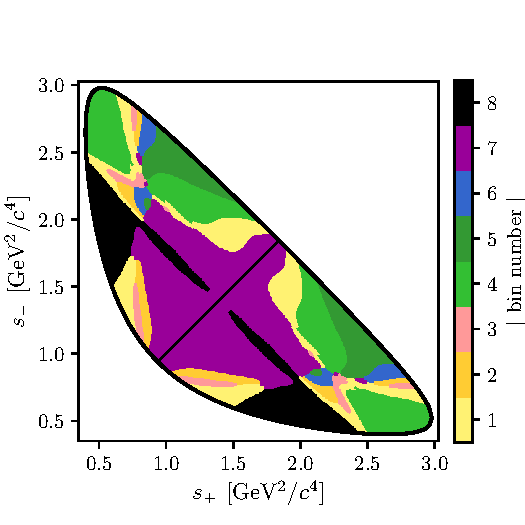
\includegraphics{figures/binning.pdf}
%     \caption{The \emph{optimal binning scheme} of the $\D\to\KS\pip\pim$ phase space~\cite{CLEOCISI}.}
%     \label{fig:optimal_binning_scheme}
% \end{figure}



% subsection a_model_independent_approach (end)

\subsection{Global CP asymmetry and the relation to GLW and ADS measurements} % (fold)
\label{sub:relation_to_glw_and_ads_measurements}



The introduction of separate normalisation factors $h^+$ and $h^-$ in Eq.~\eqref{eq:base_GGSZ_yields} hides the fact that information on $\gamma$ (in principle) can be obtained from the asymmetry in phase-space-integrated \Bp and \Bm yields. In the ideal case where $h^-=h^+$ the total yield asymmetry is 
\begin{align}\begin{split}\label{eq:A_GGSZ_global}
    A_{GGSZ} &= \frac{\sum_i N^-_- - N^+_i}{\sum_{i=-N}^N N^-i- + N^+_i}
    = \frac{ \sum_{i=-N}^N \sqrt{K_iK_{-i}}c_i (x_- - x_+)}{1 + r_B^2 +2 \sum_{i=-N}^N \sqrt{K_iK_{-i}}c_i (x_- + x_+)} \\
    &=\frac{2 \sum_{i=1}^N \sqrt{K_iK_{-i}}c_i (x_- - x_+)}{1 + r_B^2 +4 \sum_{i=1}^N \sqrt{K_iK_{-i}}c_i (x_- + x_+) },
\end{split}\end{align}
where it has been exploited that $\sum_{i=-N}^N \sqrt{K_iK_{-i}}s_i=0$ by definition. The size of the asymmetry is governed by the factor $\sum_{i=1}^N \sqrt{K_iK_{-i}}c_i$, which is small for ${\D\to\KS\pip\pim}$ and $\D\to\KS\Kp\Km$ decays. The underlying reason is that $\delta_D(\sm, \sp)$ varies significantly across phase-space for these decays, as evident by the spread in the values of $c_i$ in Tables~\ref{} and \ref{}, which reduces the \emph{average} of the asymmetry-generating \Dz--\Dzb interference term to being close to zero. As such, the value of $\sum_{i=-N}^N \sqrt{K_iK_{-i}}c_i$ is closely related to the \CP content of the final state in question: for a self-conjugate \CP even (odd) final state it is true that 
\begin{align}
    {A_\Dz(\sm, \sp)=\varpm A_\Dzb(\sm, \sp)=\varpm A_\Dz(\sp, \sm)}
\end{align}
 and thus $\sum_{i=1}^N \sqrt{K_iK_{-i}}c_i= \varpm 1$. This motivates the definition of the \CP-even fraction of the decay
\begin{align}\label{eq:Fplus_global}
    \mathcal F_+ \equiv \frac{1}{2}\left(1 + \sum_{i=1}^N \sqrt{K_i K_{-i}}c_i\right).
\end{align}
 With $\mathcal F_+$ in hand, the asymmetry in Eq.~\eqref{eq:A_GGSZ_global} can be rewritten
\begin{align}
    A_{GGSZ} &= \frac{(2\mathcal F_+-1) r_B \sin \delta_B \sin \gamma}{1 + r_B^2 (2\mathcal F_+-1) 2 r_B \cos \delta_B \cos \gamma},
\end{align}
which is the usual form used in quasi-GLW measurements~\cite{}; for $N=1$ the definition in Eq.~\eqref{eq:Fplus_global} is equivalent to $\mathcal F_+$ as defined in Ref.~\cite{}. From the definition of $K_i$ and $c_i$ it follows that the value of $\mathcal F_+$ is independent of the number and shape of bins in a given binning scheme, as long as the bin definitions follow the symmetry principles outlined in Section~\ref{}. 
For ${\D\to\KS\pip\pim}$ and $\D\to\KS\Kp\Km$ decays the values of $\mathcal F_+$ are
\begin{align}
\begin{split}
    \mathcal F_+(\KS\pip\pim) = X? \\
    \mathcal F_+(\KS\Kp\Km) = X?
\end{split}
\end{align}
as evaluated with the Belle 2018 model for ${\D\to\KS\pip\pim}$ decays and the BaBar 2010 model for $\D\to\KS\Kp\Km$ decays. Since $r_B^{\DK}\sim 0.1$ the predicted global asymmetries are thus approximately 1--2\,\%, which is not resolvable with the current experimental yields. As shown in Chapter~\ref{ch:4-KS-CPV}, \CP violation in the \KS sector leads to asymmetries of a similar size, further complicating the use of global asymmetries to constrain \xpm and \ypm. Thus these modes are ill-suited for quasi-GLW measurements, and ignoring global asymmetries leads to a negligible loss of information on $\gamma$. The reverse is true for a well-suited quasi-GLW mode, such as $\D\to\pip\pim\piz$: if $\mathcal F_+$ is close to either zero or unity, it means that $(c_i, s_i)$ will be close to $(\pm1, 0)$ in all bins for \emph{any} given binning scheme, and the set of bins will provide almost identical constraints on \xpm and \ypm. Thus, the binning of phase space leads to no gain in precision compared to a global analysis.


Indeed, a crucial quality of the GGSZ method, is that exactly because each bin-pair provides independent constraints on \xpm and \ypm, the method provides a single solution for $(\gamma, r_B, \delta_B)$ that does not suffer the ambiguities of the ADS and GLW approaches. In order to illustrate this further, it is useful to make one more comparison of the model-independent GGSZ formalism to the ADS and GLW formalisms. If there was no \CP symmetry the \Bp yield in bin $+i$ would equal the \Bm yield in bin $-i$. Therefore the relevant \CP asymmetry for a given Dalitz bin is
\begin{align}
\begin{split}
        A_{GGSZ}^i &\equiv \frac{N^-_i - N^+_{-i}}{N^-_i + N^+_{-i}} \\
    &= \frac{\sqrt{K_i K_{-i}}(c_i(\xm-\xp)+s_i(\ym-\yp))}{K_i+r_B^2K_{-i} + 2 \sqrt{K_i K_{-i}}(c_i(\xm+\xp)+s_i(\ym+\yp))}.
\end{split}
\end{align}
This expression is identical to the ADS asymmetry in Eq.~\eqref{} if the effective \D-decay parameters $r_D^i$ and $\delta_D^i$ are defined via
\begin{align}
    \kappa_i\cos\delta_D^i \equiv c_i \qquad, \qquad \kappa_i\sin \delta_D^i \equiv s_i \qquad, \qquad r_D^i \equiv \sqrt{K_i/K_{-i}},
\end{align}
and a coherence factor, $\kappa$, is included in the interference terms of the ADS expression, as is standard for multi-body \D decays~\cite{}. These parameters allow us to classify a given pair of bins with number $\pm i$ as either \emph{GLW-like}, if $ \delta_D^i$ is close to $0$ or $\pi$ and $r_D^i$  is close to unity, or \emph{ADS-like} if $0<r_D^i \ll 1$. The \CP-even fraction of the \D-decay can also be defined for a given bin-pair:
\begin{align}
\begin{split}
    \mathcal F_{+}^i = \mathcal F_+^{-i} &\equiv \frac{1}{2}\left(1 + 2c_i \frac{\sqrt{K_i K_{-i}}}{K_i + K_{-i}}\right) = \frac{1}{2}\left(1 + 2c_i \frac{r_D^i}{1+{r_D^i}^2}\right).
\end{split}
\end{align}
A GLW-even-like bin pair will have $\mathcal F_{+}^i\simeq 1$ and a GLW-even-like bin pair will have $\mathcal F_{+}^i\simeq -1$.

Table~\ref{tab:bin_categories} summarises a classification of the bins for the optimal $\DtoKspipi$ binning scheme and the 2-bins ${\DtoKskk}$ binning scheme following these principles. Two bins are classified as \emph{mixed} because $r_D^i$ is not particularly small, but $\mathcal F_+^i$ is close to 0.5. The fact that multiple bin types appear for both the \DtoKspipi and \DtoKsKK modes underline that each mode benefits from being analysed in the GGSZ formalism, and that the bins provide independent constraints that allows for a single, non-ambiguous solution for $(\gamma, r_B, \delta_B)$. 

\begin{table}
    \centering
    \caption{Classification of the bins used in model-independent GGSZ measurements, in terms of whether the interplay between the \Dz and \Dzb amplitudes in the bin resemble typical GLW or ADS behaviour. The parameters are calculated using the 2018~Belle~model~\cite{} for \DtoKspipi decays and the 2010~BaBar~model~\cite{} for \DtoKsKK decays.
    \label{tab:bin_categories}
    }
    \begin{tabular}{cccccc}
    \toprule
    \multicolumn{5}{c}{Optimal binning scheme: $\DtoKspipi$} \\
    \midrule
    Bin $i$ & $\hat r_D$ & $\hat \delta_D$ & $\mathcal F_+$ & $\kappa$ & Bin type \\
    \midrule
% autogenerated with thesis_notebooks/02_Theory/BinCategories.ipynb
    1 & $0.473$ & $    91.9^\circ$ & $48.97\,\%$ & 0.81 & Odd-even \\
    2 & $0.164$ & $    11.1^\circ$ & $63.38\,\%$ & 0.85 & ADS-like \\
    3 & $0.157$ & $    79.4^\circ$ & $52.50\,\%$ & 0.89 & ADS-like \\
    4 & $0.768$ & $   175.3^\circ$ & $5.85\,\%$ & 0.92 & GLW-odd-like \\
    5 & $0.759$ & $   -99.9^\circ$ & $42.84\,\%$ & 0.87 & Odd-even \\
    6 & $0.223$ & $   -64.5^\circ$ & $57.92\,\%$ & 0.87 & ADS-like \\
    7 & $0.651$ & $   -13.3^\circ$ & $89.44\,\%$ & 0.89 & GLW-even-like \\
    8 & $1.745$ & $    21.0^\circ$ & $87.08\,\%$ & 0.92 & GLW-even-like \\
    \midrule \\
    \midrule
    \multicolumn{5}{c}{2-bins binning scheme: $\DtoKskk$} \\
    \midrule
    Bin $i$ & $\hat r_D$ & $\hat \delta_D$ & $\mathcal F_+$ & $\kappa$ & Bin type \\
    \midrule
    % autogenerated with thesis_notebooks/02_Theory/BinCategories.ipynb
    1 & $0.816$ & $    19.8^\circ$ & $86.14\,\%$ & 0.78 & GLW-even-like \\
    2 & $0.775$ & $   154.5^\circ$ & $16.23\,\%$ & 0.77 & GLW-odd-like \\

    \bottomrule
    \end{tabular}
\end{table}

% subsection relation_to_glw_and_ads_measurements (end)




\section{Strategy for the LHCb measurement} % (fold)
\label{sec:strategy_for_lhcb_measurement}

The main topic of this thesis is a model-independent GGSZ measurement using $\BtoDK$ and $\BtoDpi$ decays, and the two \D final states $\KS\pip\pim$ and $\KS\Kp\Km$. The measurement uses the optimal binning scheme for the ${\DtoKspipi}$ mode, with the combined strong-phase inputs from the BESIII~\cite{} and CLEO~\cite{} collaborations published in Ref.~\cite{}. For the \DtoKsKK channel, the 2-bins scheme is used with the strong-phase parameters measured by the CLEO collaboration~\cite{}. The details of the analysis are presented in Chapter~\eqref{ch:5-GGSZ-measurement}, but the overall strategy and a few extensions of the formalism from the previous sections are given here.

Due to the geometry of the \lhcb detector, the signal reconstruction efficiency for $\Bpm\to\D(\to\KS h^+h^-)h'^\pm$ decays varies significantly across the \D-decay phase space. Denoting the efficiency profile as $\eta(\sm, \sp)$, the yield equations of Eq.~\eqref{eq:base_GGSZ_yields} are therefore modified slightly
\begin{align}
\begin{split}    \label{eq:lhcb_GGSZ_yields}
    N^-_i = h^\Bm \left[\Fi + \rB^2\Fmi + 2\sqrt{\Fi\Fmi}\left(\ci'\xm+\si'\ym\right)\right], \\
    N^+_i = h^\Bp \left[\Fmi + \rB^2\Fi + 2\sqrt{\Fi\Fmi}\left(\ci'\xp-\si'\yp\right)\right],
\end{split}
\end{align}
where the phase-space integrated quantities now include the efficiency profile
\begin{align}\label{eq:Fi_def}
    F_i &= \frac{1}{N_F}\int_i\text{d}s^2 \,\eta(\smp)|\ADS(\smp)|^2, &
    N_F &=\int\text{d}s^2 \,\eta(\smp)|\ADS(\smp)|^2,
\end{align}
\begin{align}\label{eq:ci_si_with_eff}
\begin{split}
    \ci' &= \frac
    {\int_i \text{d}s^2 \,\eta(\smp)|\ADS(\smp)||\ADS(\spm)|\cos[\delta_D(\smp)]}
    {\sqrt{\int_i \text{d}s^2 \,\eta(\smp)|\ADS(\smp)|^2}\sqrt{\int_i \text{d}s^2 \,\eta(\smp)|\ADS(\spm)|^2}},
\end{split}
\end{align}
with an analogous definition of $\si'$. At leading order, the strong-phase parameters are unaffected by the non-uniform efficiency, and, in addition, the bin definitions favour bins for which $c_i$ and $s_i$ take on similar values across each bin.  Therefore, the reported \ci and \si values are used directly in the measurement. The impact on the obtained central values is negligible, as described in detail in Section~\ref{} where a systematic uncertainty is assigned. 

The \Fi \emph{are} significantly different to the $K_i$ due to the experimental acceptance profile in \lhcb. Given external inputs for the strong-phase parameters, it is possible to fit the \Fi parameters \emph{and} $\xpm$ and $\ypm$ simultaneously in a fit to the \lhcb \BtoDK data set, in which case the obtained \Fi parameters incorporate the correct acceptance profile correction by construction. However, the obtainable precision for the \CP observables measured by this procedure is suboptimal. As an alternative, the first \lhcb measurement made a simultaneous analysis of \BtoDK and a much larger sample of \BtoDpi decays; since the \Fi parameters relate to the \D decay, they can effectively be obtained in the \Dpi sample  and shared between the two \BtoDh channels. However, there is \CP violation present in the \BtoDpi decays, which led to a dominant systematic uncertainty. Later \lhcb measurements instead relied on flavour tagged \D mesons from $\Bzb\to\Dstarp(\to \Dz \pip)\mu^- \bar \nu_\mu X$ decays, where no \CP violation in possible, to obtain \Fi. However, due to necessarily different triggering paths and selections, the acceptance profile is not exactly identical between semi-leptonic decays and the \BtoDh decays of interest. An efficiency correction based on simulation was therefore applied to obtain the correct \Fi; the uncertainty related to the correction constituted the largest systematic uncertainty to the measurement~\cite{}.

Both sources of systematic uncertainty can be avoided by making a simultaneous analysis of \BtoDK and \BtoDpi decays, where \CP-violating observables are measured in \emph{both} channels and the \Fi parameters are shared. Effectively, the \Fi are determined in the high statistics \BtoDpi channel, but with no systematic effect from \CP-violation in that channel, since the \CP-violation is incorporated in the yield description. At the start of the work that lead to this thesis, it was not clear to what degree the measured \CP-violating observables in \BtoDpi decays were affected by \CP violation in the neutral kaon sector. The impact had been shown to scale as $\mathcal O(|\epsilon| / r_B)$~\cite{}, which is negligible for the \BtoDK channel but suggests potentially large biases in the \BtoDpi channel, where $r_B$ is $~20$ times smaller. However, the dedicated analysis presented in Chapter~\ref{ch:4-KS-CPV} has proved the effect on GGSZ measurements to be in fact be \emph{smaller} than $\mathcal O(|\epsilon| / r_B)$ and the simultaneous measurement is indeed viable. 

The measurement is performed, by making extended maximum-likelihood fits to the $m_B$ spectra of $\B\to\D(\to\KS h^+h^-)\Kpm$ candidates split by charge and Dalitz bin, where the signal yields are parameterised using the expressions in Eq.~\eqref{}, thus obtaining values for \xpmdk and \ypmdk directly. 
The Cartesian \CP-violating observables \xpm and \ypm are employed because they lead to better statistical behaviour than fits to data where the underlying parameters $(\gamma, r_B^\DK, \delta_B^\DK)$ are determined~\cite{}, at the cost of introducing a fourth degree of freedom. 

With the addition of the \BtoDpi mode as a true signal channel, two new underlying parameters are introduced, $r_B^{\DPi}$ and $\delta_B^{\DPi}$. It is only necessary to introduce an additional two, not four, Cartesian parameters~\cite{} by defining
\begin{subequations}
\begin{align}
    \xi_{\DPi} = \left(\frac{r_B^{\DPi}}{r_B^{\DK}}\right)\exp [i (\delta_B^{\DPi}-\delta_B^{\DK})]
\end{align}
and letting
\begin{align}
    \xxidpi &= \Re [\xi_{\Dpi}] & \yxidpi &= \Im [\xi_{\Dpi}].
\end{align}
\end{subequations}
In terms of these parameters, the usual Cartesian \xpm and \ypm are given by
\begin{align}\label{eq:xy_from_xi}
    x_\pm^{\D\pi} &= x_\xi^{\D\pi}x_\pm^{DK} - y_\xi^{\D\pi}y_\pm^{DK}, 
    & y_\pm^{\D\pi} &= x_\xi^{\D\pi}y_\pm^{DK} + y_\xi^{\D\pi}x_\pm^{DK}.
\end{align} 
Using this expression, the \BtoDpi yields can also be defined via Eq.~\eqref{} in the maximum-likelihood fit. This allows for a stable fit for all six $x$ and $y$ parameters, as well as the shared \Fi, as described in much greater detail in Chapter~\ref{}. Note that $\xi$ does not depend on $\gamma$: all information on \CP asymmetries in both the \BtoDK and \BtoDpi channels is encoded in \xpmdk and \ypmdk. 

The combined analysis of \BtoDK and \BtoDpi decays presents a significant step forward, because it solves the problem of obtaining \Fi parameters for the appropriate acceptance profile in a manner that avoids leading systematic uncertainties, and almost all reliance on simulation. This is of great importance, if the large data samples that will be collected by \lhcb in the future are to be exploited to their full potential.


% subsection measuring_strong_phase_inputs_at_charm_factories (end)


% subsection extending_the_method_to_multiple_decay_channels (end)

% section the_ggsz_method(end)

% section cp_violation_in_the_standard_model (end)